\documentclass[compress, hyperref={pdfpagelayout=SinglePage}]{beamer}

%Para digitar e compreender em portugues os comandos
\usepackage[spanish]{babel}
\usepackage[utf8]{inputenc}

\usepackage{verbatim}

%Remove Warnings de tamanho de letra.
\usepackage{lmodern} 

%Pacote de cores
\usepackage{color}
\usepackage{xcolor}   
\usepackage{colortbl}

\definecolor{verde}{rgb}{0.88,1,1}
\definecolor{azul}{rgb}{0.62, 0.85, 1}
\definecolor{amarelo}{rgb}{1, 0.95, 0.62}
\definecolor{vermelho}{rgb}{0.85, 0, 0.075}
\definecolor{roxo}{rgb}{0.69, 0.57, 0.86}


%Seleciona um tema para usar na apresentação.
\usetheme{CambridgeUS}

%Remove a barra de navegacao(bugada) do Beamer.
\setbeamertemplate{navigation symbols}{}

%Permite utilizar hyperlinks externos
\usepackage{hyperref}
\hypersetup{linkcolor=blue,citecolor=blue,filecolor=black,urlcolor=MidnightBlue} 

%Primeiro paragrafo eh identado
\usepackage{indentfirst}

%Otimizacao de tabelas/espacamento/pdf
\usepackage{array}  
\usepackage{microtype}
\usepackage{cmap}
\usepackage[T1]{fontenc}

%Parece letra times
\usepackage{times}
\usepackage{graphicx}


\title[Presentacion Univ. Andes]{Desarrollo de técnicas para recomendar actividades en flujos de trabajo científicos: un enfoque basado en ontologías.}
\author{Alumno: Adilson Lopes Khouri}

\institute[USP]{Orientador: Prof. Dr. Luciano Antonio Digiampietri}

\begin{document}

\begin{frame}
  \titlepage
\end{frame}

\section*{Resumen}

\begin{frame}{Resumen}
  \tableofcontents
\end{frame}

\section{Introducción}

\begin{frame}		
	\begin{block}{Introducción}
		 \begin{enumerate}
		  \item \emph{e-Science}.
		  \item Sistemas de gestión de flujos de trabajo científicos.
			  \begin{itemize}
			  	\item Ver grandes cantidades de datos.
				\item Cálculos matemáticos.
				\item Análisis del genoma.
			  \end{itemize}
		  \item Evitar escribir funciones/métodos existentes.
		  \item Gran cantidad de actividades.
		  \item Sistema para recomendar actividades.
		 \end{enumerate}
	\end{block}
\end{frame}
\section{Objetivos}
	\begin{frame}
		\begin{block}{Objetivo general}
			Este grado de maestria tiene como objetivo especificar e implementar una técnica de recomendación de actividad en flujos de trabajo científicos que combine: 
				\begin{enumerate}
					\item Ontologías
					\item Frecuencia de pares de actividades
					\item Actividades de entrada y salida
				\end{enumerate}
		\end{block}
	\end{frame}

\begin{frame}
	\begin{block}{Objetivos específicos}
		\begin{enumerate}
			\item Construya una base de datos de flujos de trabajo científicos
			\item Modelado de recomendaciones de actividad como un problema de clasificación/regresión
			\item Comparación entre diferentes técnicas de literatura y soluciones propuestas
		\end{enumerate}
	\end{block}
\end{frame}
\section{Conceptos Fundamentales}

\begin{frame}
	\begin{block}{Conceptos Fundamentales}
		 \begin{enumerate}
		  \item Sistemas de gestión de flujos de trabajo científicos.
		  \item Sistemas de recomendación.
		  \item Recomendación sobre flujos de trabajo científicos.
		  \item Ontologías.
		  \item Recomendación basada en bases de datos de flujos de trabajo científicos.
		  \item Validación de métricas.
		  \item Recomendación de la base de datos de flujo de trabajo.
		  \item Clasificadores y regresores.
		 \end{enumerate}
	\end{block}
\end{frame}


\begin{frame}
	\begin{figure}[!htb]
		\centering	  				
		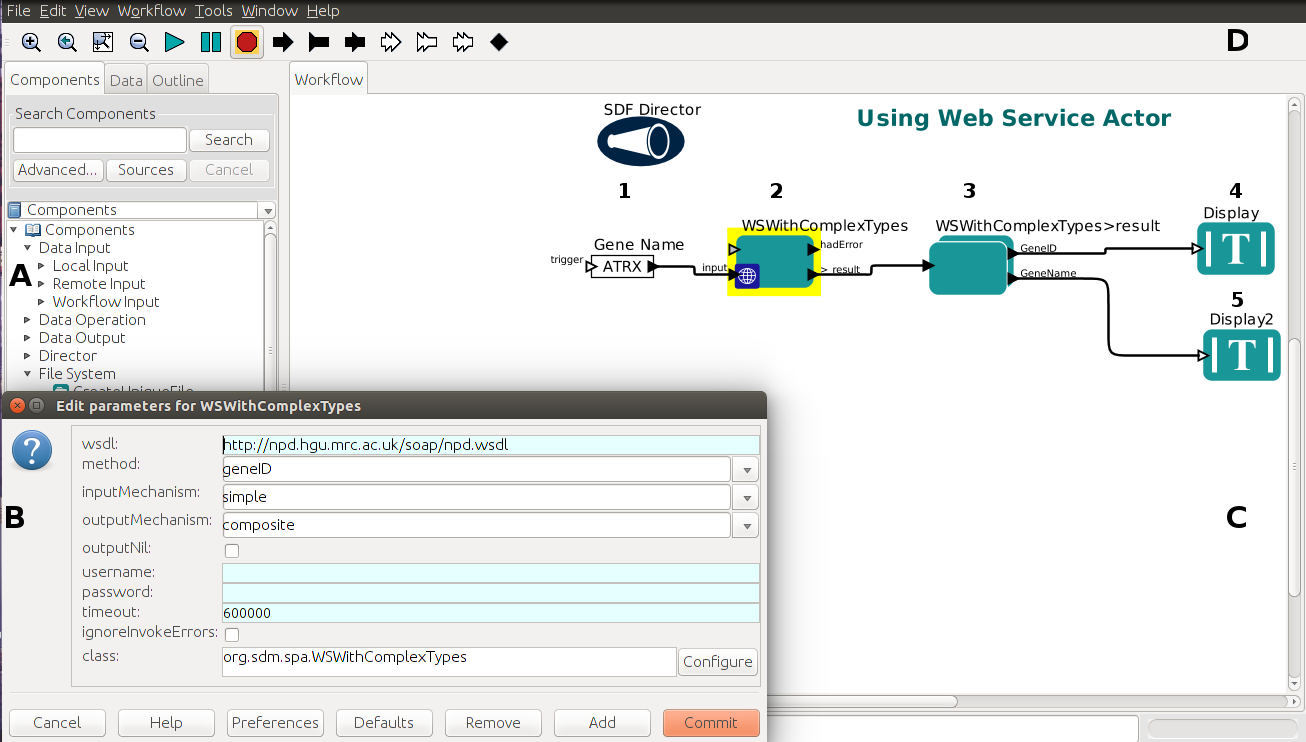
\includegraphics[height=7cm]{./secoes/ConceitosFundamentais/webService.png}
		\caption{Ejemplo de sistema de gestión de flujo de trabajo científico.}
		\label{fig_sistema_gerenciador_workflow_cientifico}
 	\end{figure}
\end{frame}


\begin{frame}		
	\begin{block}{}
		Los sistemas de recomendación están destinados a \textbf{recomendar elementos útiles} a los usuarios:
		\begin{eqnarray}
		\forall c \in C,  \quad s_{c}^{'} =  \operatorname*{arg\,max}_{s \in S} u(c,s) \label{formalizar_recomendacao}
		\end{eqnarray}
		
%		A função utilidade \(u\) não está definida para todo o espaço \(C \times S\), isso força os sistemas de recomendação a extrapolar o espaço conhecido.
		La función de utilidad \(u\) no está definida para todo el espacio \(C \times S\), esto obliga a los sistemas de recomendación a extrapolar el espacio conocido.
	\end{block}
\end{frame}


\begin{frame}
	\begin{block}{}
		Algunas estrategias utilizadas en los sistemas de recomendación:
		
		\begin{enumerate}
			\item \emph{Content-based}
			\item \emph{Collaborative Filter (usuarios similares)}
			\item \emph{Hibrid Approach}
			\item \emph{Community Based (usuarios amigables)}
			\item \emph{Demographic}
			\item \emph{Knowledge-based}
		\end{enumerate}
	\end{block}
\end{frame}


\begin{frame}		
	\begin{block}{}
		\textbf{Recomendar actividades en flujos de trabajo científicos} requiere, además de la extrapolación mencionada anteriormente, considerar las restricciones:
		\begin{enumerate}
			\item Dependencia entre entrada y salida de actividades
			\item Dependencia semántica
			\item El orden de las actividades
		\end{enumerate}
	\end{block}
\end{frame}


\begin{frame}
	\begin{block}{}
		\textbf{Ontology} es un modelo para la representación del conocimiento, que se puede utilizar para anotar semánticamente actividades.
		
		\begin{figure}
			\begin{minipage}[b]{0.7\textwidth}
				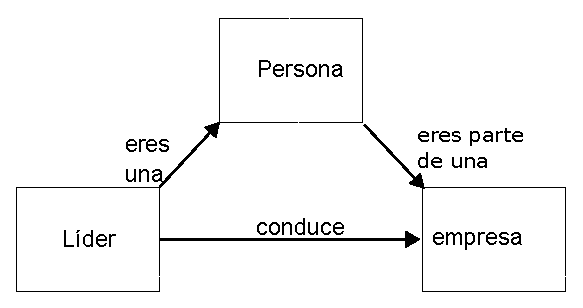
\includegraphics[width=\textwidth]{./secoes/ConceitosFundamentais/Ontologia.eps}
				\caption{Ejemplo de ontología}
			\end{minipage}
		\end{figure}
	\end{block}
\end{frame}

\begin{frame}
	\begin{block}{}
		Los experimentos serán validados por \emph{validación cruzada 10 veces}, cada ronda calculará las métricas:
		\begin{enumerate}
			\item \emph{Sucess at rank k} (\(S@k\)).
			\item \emph{Mean Reciprocal Rank} (MRR).		
		\end{enumerate}
		
		\begin{figure}
			\begin{minipage}[b]{0.9\textwidth}
				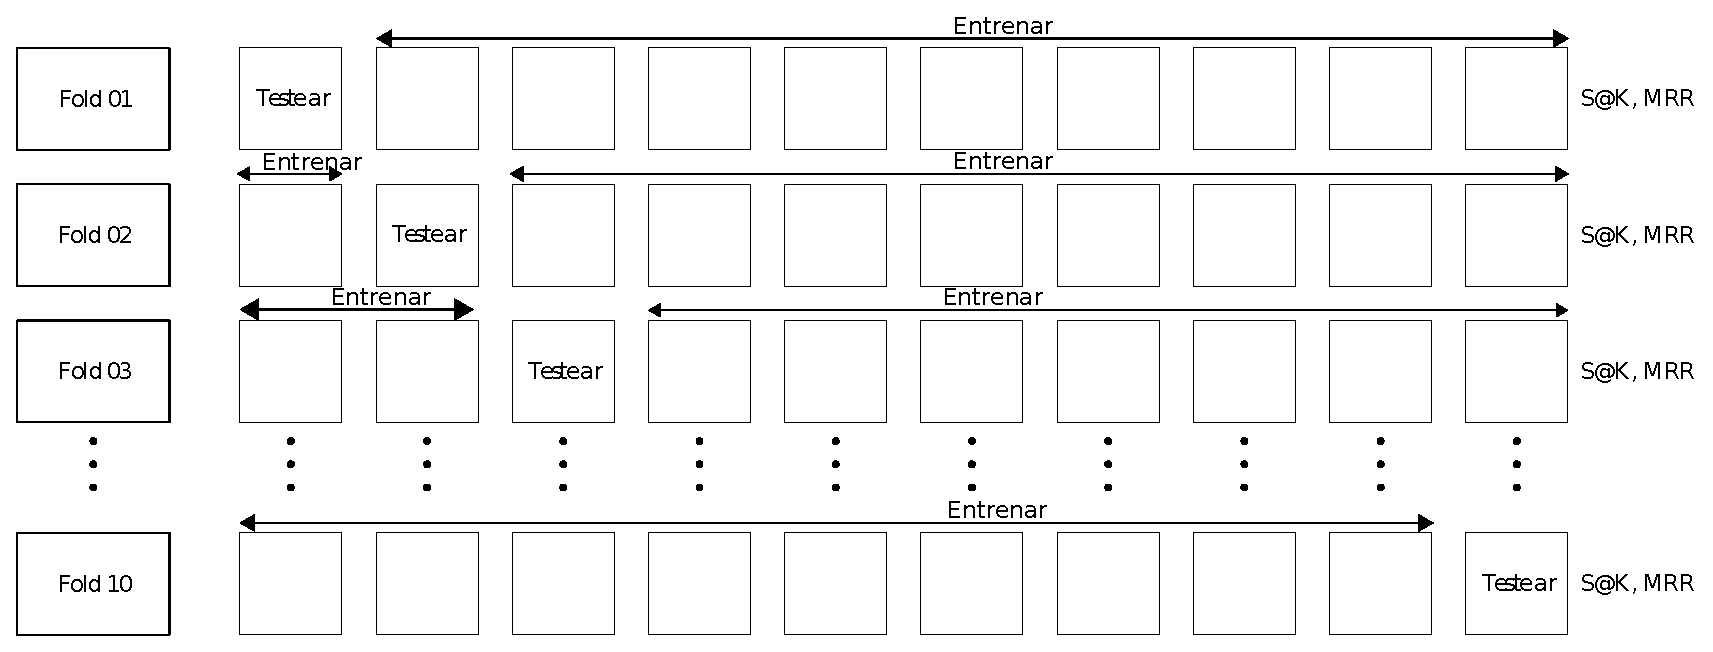
\includegraphics[width=\textwidth]{./secoes/ConceitosFundamentais/10FOLDCROSS.eps}
				\caption{Exemplo de \emph{10-fold cross validation}}
			\end{minipage}
		\end{figure}
		
	\end{block}
\end{frame}

\begin{frame}
	\begin{block}{}
		\textbf{Recomendación de base de datos de flujo de trabajo}
		\begin{enumerate}
			\item Frecuencia
			\item \emph{itemsets}.	
		\end{enumerate}
	\end{block}
\end{frame}


\begin{frame}
	\begin{block}{}
		\textbf{Recomendación de clasificadores}
		\begin{enumerate}
			\item CART;
			\item KNN;
			\item Naive Bayes;
			\item Rede Neural (MLP);
			\item SVM (C-SVM).		
		\end{enumerate}
	\end{block}
\end{frame}

\begin{frame}
	\begin{block}{}
		\textbf{Recomendación de los regresores}
		\begin{enumerate}
			\item CART;
			\item MARS;
			\item Binomial;
			\item Rede Neural (MLP);
			\item SVM (\(\epsilon\)-SVM).		
		\end{enumerate}
	\end{block}
\end{frame}

\begin{frame}
	\begin{block}{}
		\textbf{Recomendación de clasificadores compuestos}
		\begin{enumerate}
			\item SVM;
			\item Rotation Forest.		
		\end{enumerate}
	\end{block}
\end{frame}

\section{Revisión sistemática}

\begin{frame}		
	\begin{block}{Revisión sistemática}
		La revisión de la literatura empezó con un estudio exploratorio seguido de una revisión sistemática. Por lo tanto, fue posible:
		\begin{enumerate}
			\item Encontrar un área de recomendación de vanguardia para flujos de trabajo científicos.
			\item Comprender el problema.
			\item Encuentrar términos específicos del área.
			\item Definir palabras clave
		\end{enumerate}
	\end{block}
\end{frame}

\begin{frame}		
	\begin{block}{Conducir}
		\begin{figure}
			\tiny
			\begin{minipage}[b]{0.46\textwidth}
				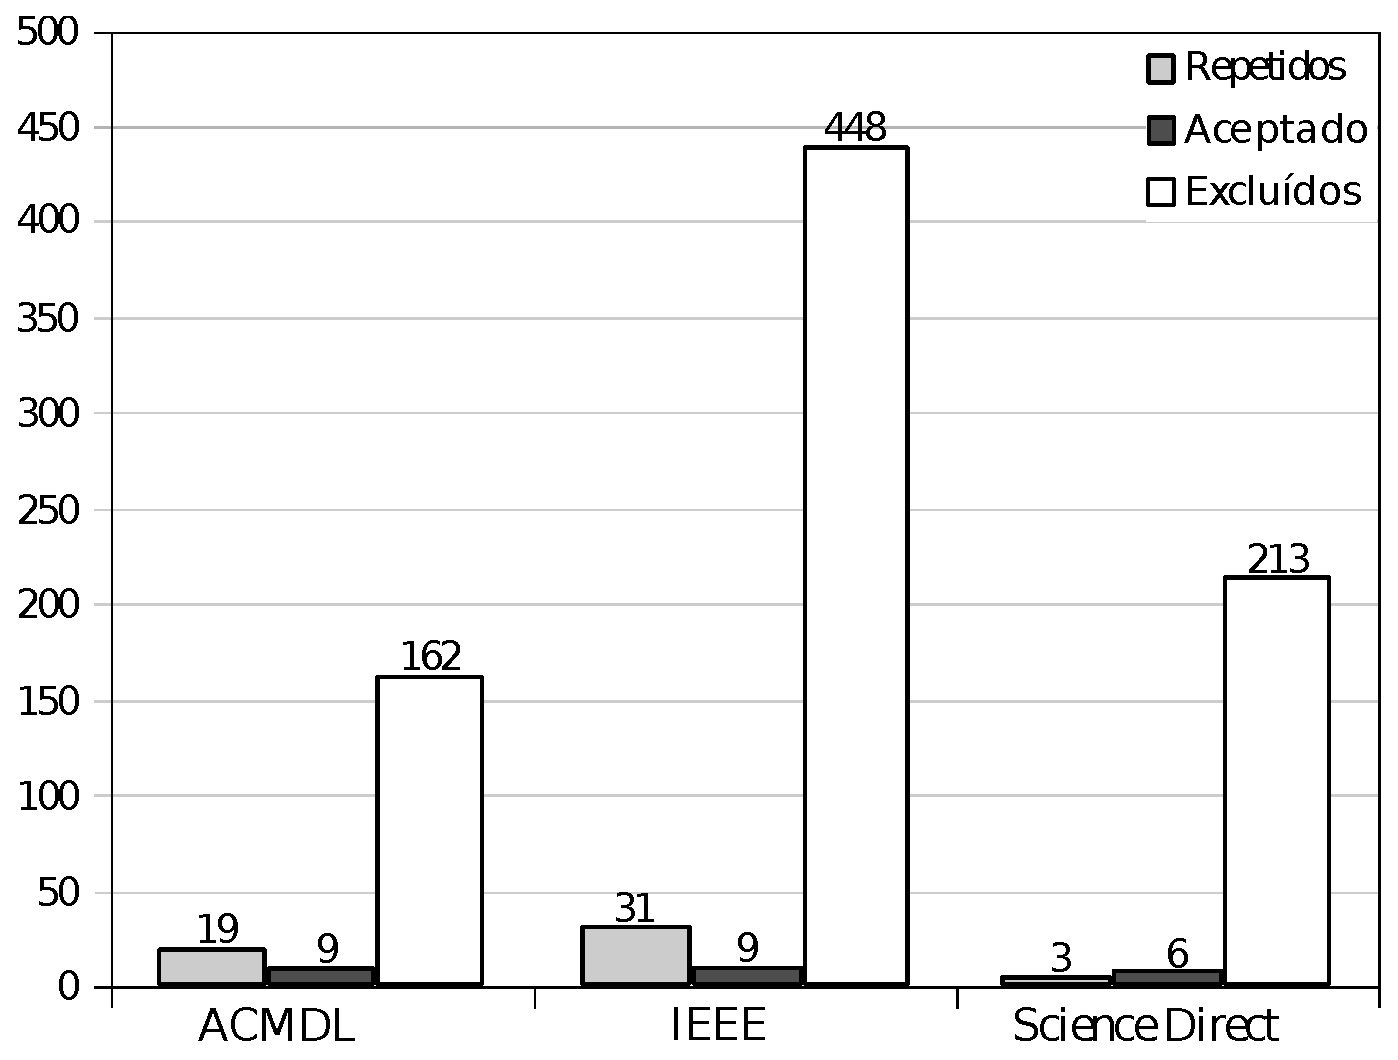
\includegraphics[width=\textwidth]{./secoes/RevisaoDaLiteratura/GraficoQuantidade.eps}
				\caption{Número de artículos por técnica.}
			\end{minipage}
			%\qquad
		     \hspace{0.1cm}
			\begin{minipage}[b]{0.46\textwidth}
				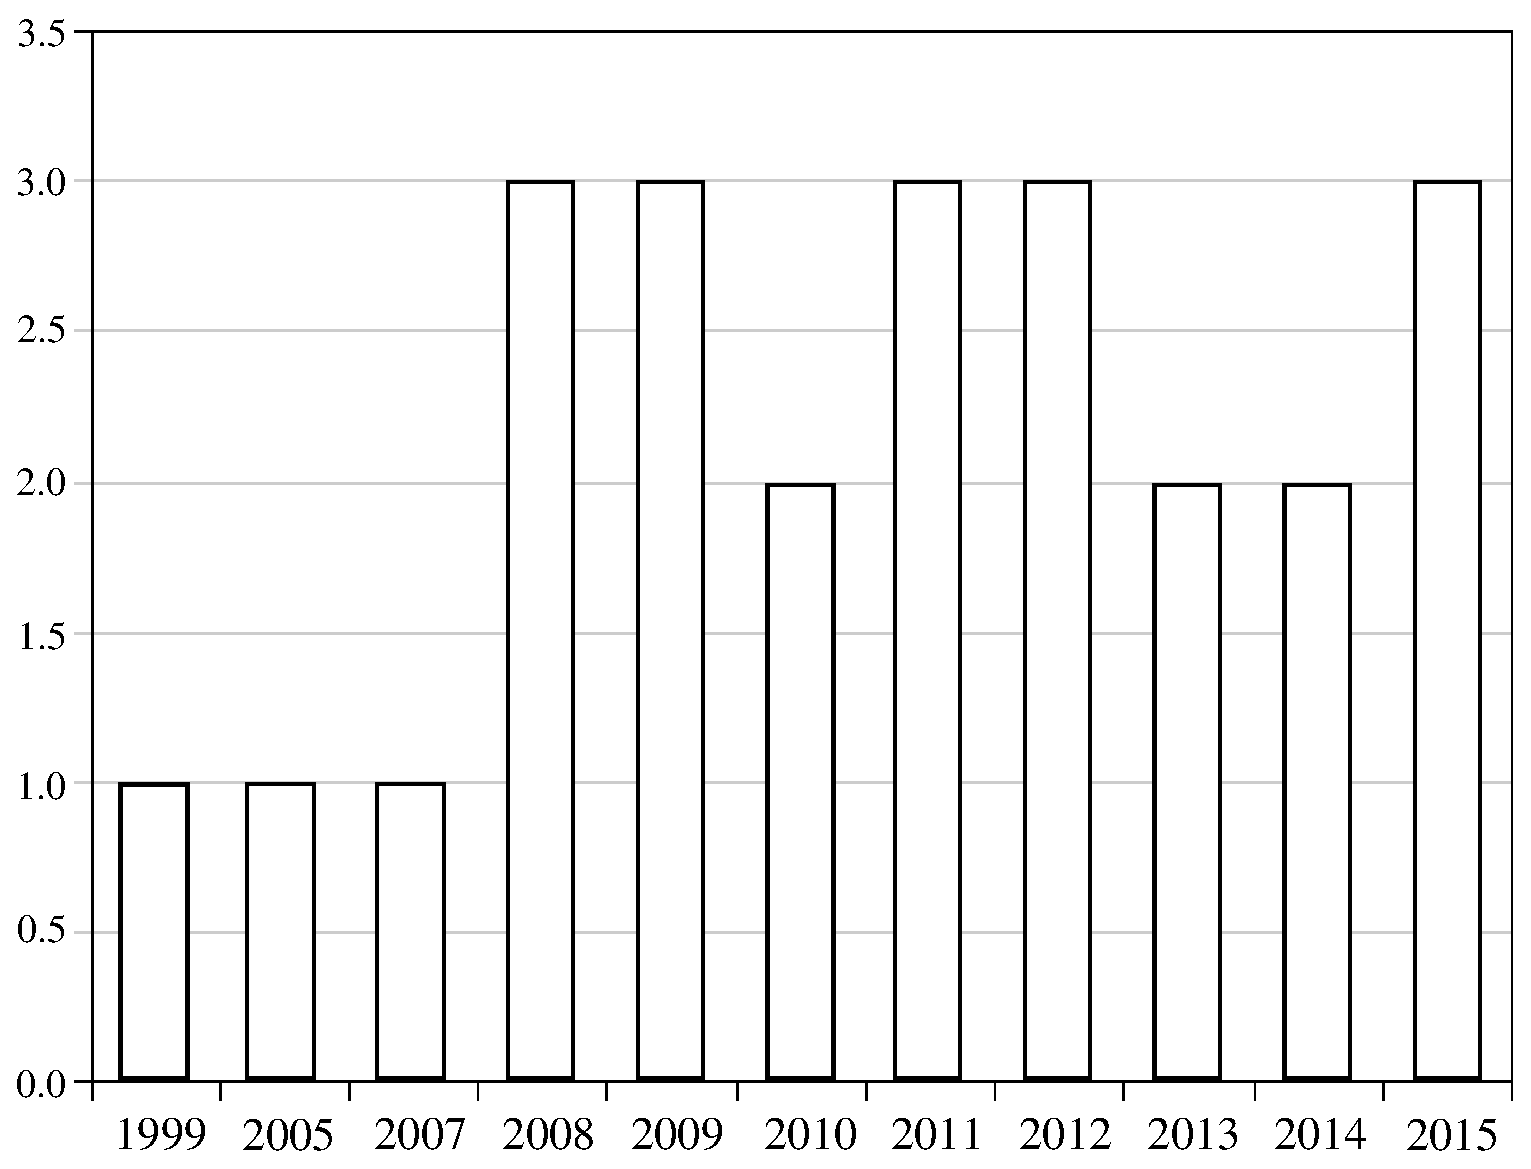
\includegraphics[width=\textwidth]{./secoes/RevisaoDaLiteratura/GraficoQuantidadeAno.eps}
				\caption{Artículos por año de publicación}
			\end{minipage}
		\end{figure}
		
	\end{block}
\end{frame}

\begin{frame}		
	\begin{block}{Ejecución}
		Se observa que la técnica de procedencia es la más utilizada seguida de: i) Frecuencia; ii) entrada y salida; iii) \emph{itemsets}; y iv) ontologías.
		\begin{figure}
			\begin{minipage}[b]{0.5\textwidth}
				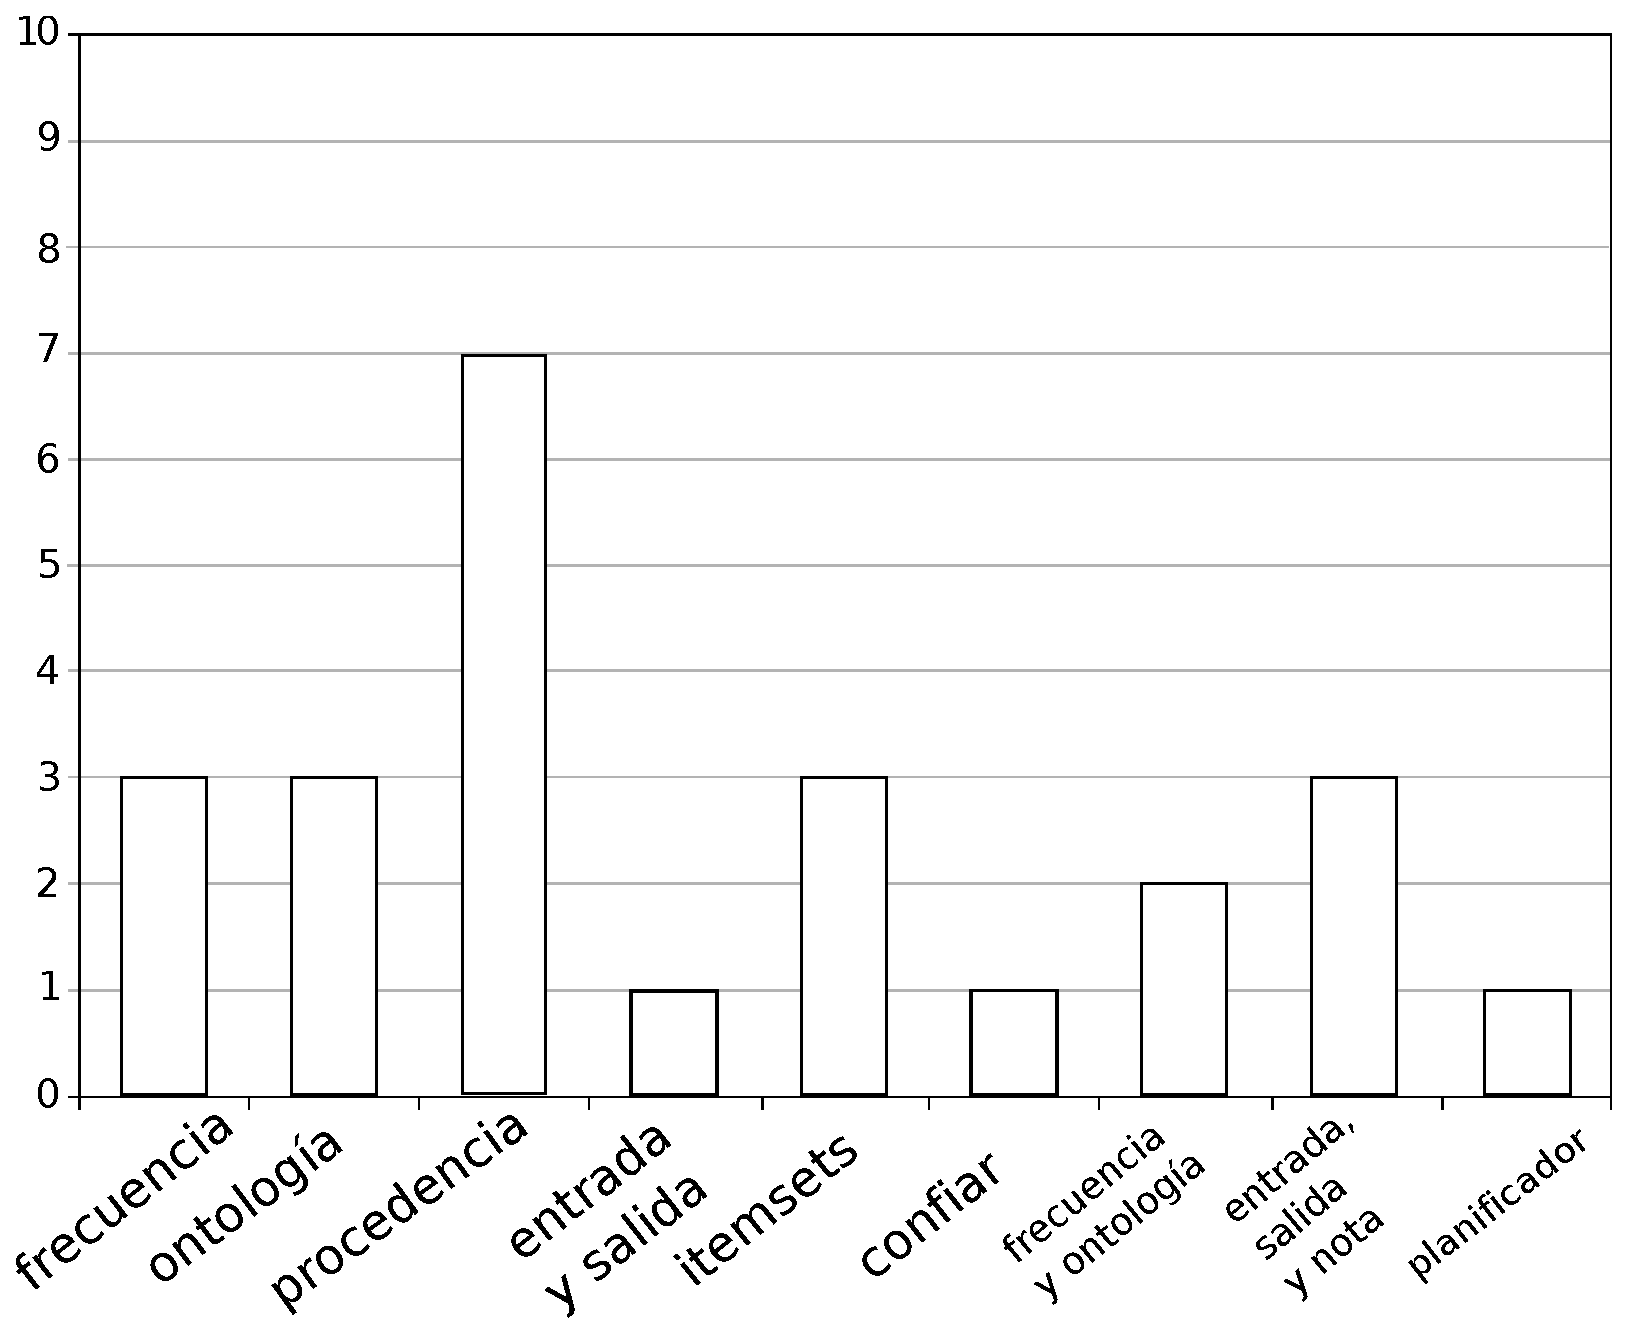
\includegraphics[width=\textwidth]{./secoes/RevisaoDaLiteratura/GraficoQuantidadeTecnica.eps}
%				\caption{Número de artículos por técnica.}
			\end{minipage}
		\end{figure}
		
	\end{block}
\end{frame}

\begin{frame}		
	\begin{block}{Comparación de la técnica propuesta con la literatura relacionada.}
		Las principales ventajas de la técnica propuesta, en relación con las de la literatura relacionada, son considerar las dependencias de entrada y salida, la semántica y la frecuencia de las actividades. 
		
		Además, no se requieren datos de procedencia, redes sociales, recomendacion por confianza entre usuarios o tipo de actividad: i) Shim; ii) Simples; I/O iii) Subflujo de trabajo.
	\end{block}
\end{frame}


\section{Solución propuesta}

\begin{frame}		
	\begin{block}{Solución propuesta}
		La solución propuesta en este Máster recomienda actividades que utilizan tres conceptos importantes en el área de los flujos de trabajo científicos: i) frecuencia de las actividades; ii) compatibilidad entre entrada y salida; y ii) semántica de actividad
	\end{block}
\end{frame}


\begin{frame}		
	\begin{block}{Desarrollo de ontologías}
		La ontología se desarrolló utilizando la metodología \emph{Skeletal}, que contiene las siguientes fases:
		\begin{enumerate}
			\item Identificar el propósito
			\item Construcción de ontologías:
			\begin{enumerate}
				\item Captura de ontologías
				\item Codificación de ontología;
				\item Integración con ontologías existentes
			\end{enumerate}
			\item Validación
			\item Documentación
		\end{enumerate}
	\end{block}
\end{frame}


\begin{frame}		
	\begin{block}{Matriz de técnicas de literatura}
		\begin{table}[htb]
			\centering
			\caption{Ejemplo de matriz de entrada para técnicas de literatura relacionadas}
			\begin{tabular}{|c|c|c|c|c|}  \hline
				\textbf{\emph{Workflow}} & \textbf{Activ \(\mathbf{01}\)} & \textbf{Activ \(\mathbf{02}\)} & \textbf{\(\mathbf{\ldots}\)} & \textbf{Activ \(\mathbf{280}\)}  \\ \hline
				01 			  & 1 			  & 0 			  & \(\ldots\) 	  & 0  				\\ \hline
				02 			  & 1 			  & 1 			  & \(\ldots\) 	  & 1  				\\ \hline
				03 			  & 1 			  & 0 			  & \(\ldots\) 	  & 1  				\\ \hline
				\(\vdots\) 		  			  & \(\vdots\) 	  & \(\vdots\) 	  & \(\vdots\) 	  & \(\vdots\) 		\\ \hline
				73 			  & 1 			  & 0 			  & \(\ldots\) 	  & 0  				\\ \hline
			\end{tabular}
			\label{tabela_matriz_de_dados}
			%\vspace{0.1cm}
			%\source{\varAutorData}
		\end{table}
	\end{block}
\end{frame}


\begin{frame}		
	\begin{block}{Matriz para técnicas de clasificación}
		Las actividades más comunes que se utilizan para garantizar el equilibrio del clasificador en el que se replican, son \(59\) 
		\begin{table}[!htb]
			\footnotesize
			\centering
%			\caption{Ejemplo de matriz de entrada para técnicas de classificación y regreción}
			\begin{tabular}{|c|c|c|c|c|c|c|c|c|}  \hline
				\textbf{\(\#\)} & \textbf{\emph{Workflow}} & \textbf{Ativ \(\mathbf{01}\)} & \textbf{Activ \(\mathbf{02}\)} & \textbf{\(\mathbf{\ldots}\)}  & \textbf{Activ \(\mathbf{279}\)} & \textbf{Activ \(\mathbf{280}\)} & \textbf{Etiqueta} \\ \hline
				
				1	&		01		 			   & 1 			  & 0 			  & \(\ldots\) 	  & 0 & 0  			& T	\\ \hline
				2	&		01 					   & 1 			  & 0 			  & \(\ldots\) 	  & 0 & 0  			& T	\\ \hline
				\(\vdots\)  &  \(\vdots\) 	   	   & \(\vdots\)   & \(\vdots\) 	  & \(\vdots\) 	  & \(\vdots\) & \(\vdots\) & \(\vdots\)\\ \hline
				59	&		01 					   & 1 			  & 0 			  & \(\ldots\) 	  & 0 & 0   		& T	\\ \hline
				1	&		01		 			   & 0 (eliminado) 		  & 1 (añadido) &\(\ldots\)& 1 & 0	& F	\\ \hline
				2	&		01 					   & 0 (eliminado)& 0 		  & \(\ldots\) 	  & 1 (añadido) & 0& F	\\ \hline
				\(\vdots\)  &		\(\vdots\) 	   & \(\vdots\) & \(\vdots\) 	  & \(\vdots\) 	  & \(\vdots\) & \(\vdots\) & \(\vdots\) \\ \hline
				59	&		01 					   & 0 (eliminado)			  & 0 			  & \(\ldots\) & 0 & 1 (añadido)& F \\ \hline
				&\(\vdots\) & & & & & & 																		\\ \hline
				1	&		73		 			   & 1 			  & 1  & \(\ldots\) 	  & 0 & 0  			& T	\\ \hline
				2	&		73 					   & 1 			  & 1  & \(\ldots\) 	  & 0 & 0  			& T	\\ \hline
			\end{tabular}
			\label{tabela_matriz_de_dados_adapatada_classificacao_regressao}
		\end{table}
	\end{block}
\end{frame}


\begin{frame}		
	\begin{block}{Técnica propuesta}
		Para explicar la técnica propuesta se utilizará la figura:
				\begin{figure}
					\begin{minipage}[b]{0.8\textwidth}
						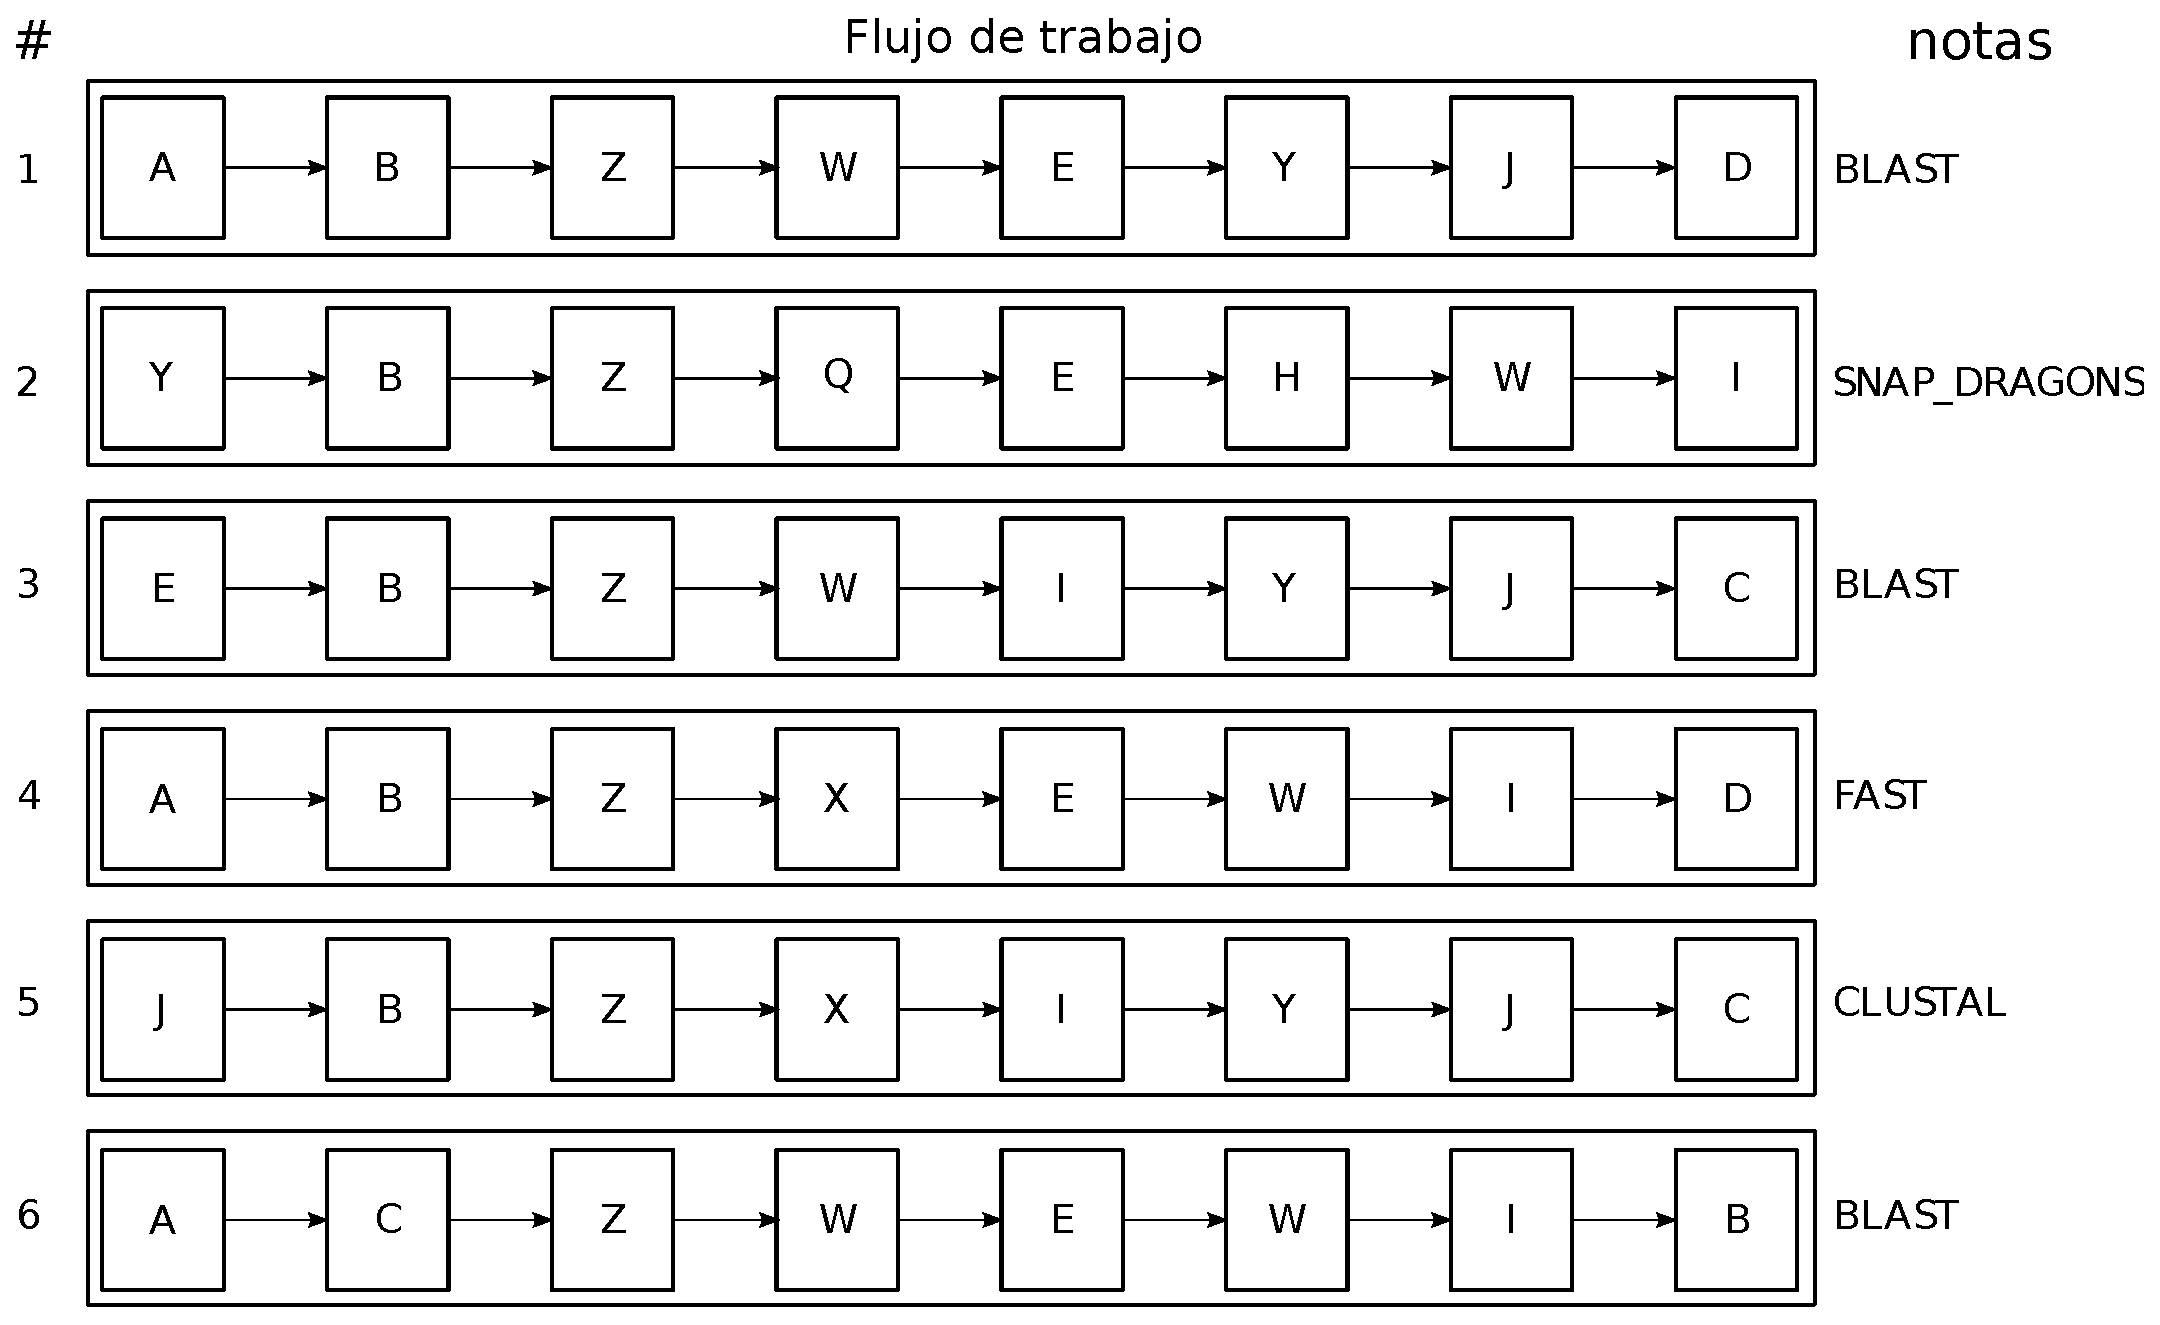
\includegraphics[width=\textwidth]{./secoes/SolucaoProposta/recomendacaofreqontologia.eps}
						\caption{Ejemplo de base de datos de flujos de trabajo científicos}
					\end{minipage}
				\end{figure}
	\end{block}
\end{frame}


\begin{frame}		
	\begin{block}{Técnica propuesta}
		Recomendación para la actividad \emph{Z} ordenada por frecuencia y concepto ontológico.
		\begin{table}[!htb]
			\centering
			%\caption{Recomendação para a atividade \emph{Z} ordenada por frequência e conceito ontológico}
			\begin{tabular}{|c|c|c|c|}  \hline
				\textbf{Posición de la lista} & \textbf{Activ} & \textbf{Frecuencia} & \textbf{Actividad de notas} 	\\ \hline
				1				& W 				& 3 				& BLAST				\\ \hline
				2				& X 				& 2 				& FAST, CLUSTAL		\\ \hline
				3				& Q 				& 1 				& SNAP DRAGONS		\\ \hline
				\(\vdots\)		& \(\vdots\)		& \(\vdots\) 		& \(\vdots\)		\\ \hline
				280				& \(\vdots\)		& \(\vdots\)		& \(\vdots\)	\\ \hline
			\end{tabular}
			\label{tabela_lista_recomendacao_ordenada_frequencia}
			%\vspace{0.1cm}
			%\source{\varAutorData}
		\end{table}		
	\end{block}
\end{frame}
\section{Comparación de experimentos}

\begin{frame}		
	\begin{block}{Comparación de experimentos}
		Resultados de los sistemas de recomendación.
		\bgroup
		\begin{table}[!htp]
			\centering
			\tiny
			\begin{tabular}{|l|l|l|l|l|l|l|l|l|} \hline
				\textbf{\(\mathbf{\#}\)} & \textbf{Técnica}&\textbf{S@1}&\textbf{S@5} & \textbf{S@10} & \textbf{S@50} & \textbf{S@100} & \textbf{S@280} & \textbf{MRR} \\ \hline
				
\rowcolor{roxo}		1  & Random				& 0,0037 & 0,0260 & 0,0280 & 0,0300 & 0,0400 & 1,0000 & 0.033 \\ \hline
\rowcolor{roxo}		2  & \emph{Apriori}			& 0,0037 & 0,0385 & 0,0559 & 0,0568 & 0,0570 & 1,0000 & 0,037 \\ \hline
\rowcolor{amarelo}	3  & KNN\(_C\)				& 0,0037 & 0,0685 & 0,0959 & 0,5068 & 1,0000 & 1,0000 & 0,040 \\ \hline
\rowcolor{amarelo}	4  & Rede neuronal\(_C\)		& 0,0137 & 0,1507 & 0,1781 & 0,8082 & 1,0000 & 1,0000 & 0,089 \\ \hline
\rowcolor{amarelo}	5  & CART\(_C\)				& 0,0274 & 0,1233 & 0,3699 & 0,7671 & 1,0000 & 1,0000 & 0,113 \\ \hline
\rowcolor{amarelo}	6  & Naive Bayes\(_C\)     	& 0,0274 & 0,1507 & 0,3425 & 0,6301 & 1,0000 & 1,0000 & 0,114 \\ \hline
\rowcolor{verde}	7  & Binomial\(_R\) 		& 0,0822 & 0,1918 & 0,2055 & 0,8493 & 1,0000 & 1,0000 & 0,136 \\ \hline
\rowcolor{verde}	8  & Rede neuronal\(_R\)     	& 0,1096 & 0,2603 & 0,2603 & 0,2603 & 1,0000 & 1,0000 & 0,154 \\ \hline
\rowcolor{verde}	9  & MARS\(_R\)     		& 0,1233 & 0,2055 & 0,2192 & 0,7260 & 1,0000 & 1,0000 & 0,167 \\ \hline
\rowcolor{verde}	10 & SVM\(_R\)     			& 0,1233 & 0,3151 & 0,4932 & 0,8493 & 1,0000 & 1,0000 & 0,238 \\ \hline
\rowcolor{verde}	11 & CART\(_R\)    			& 0,1370 & 0,1370 & 0,2603 & 0,6164 & 1,0000 & 1,0000 & 0,114 \\ \hline
\rowcolor{roxo}		12 & FES           			& 0,1474 & 0,2603 & 0,3699 & 0,8671 & 1,0000 & 1,0000 & 0,196 \\ \hline
\rowcolor{amarelo}	13 & SVM\(_C\)    			& 0,2425 & 0,4658 & 0,4932 & 0,7123 & 1,0000 & 1,0000 & 0,244 \\ \hline
\rowcolor{azul}		14 & SVM composto\(_C\)		& 0,2515 & 0,4458 & 0,5232 & 0,7623 & 1,0000 & 1,0000 & 0,314 \\ \hline
\rowcolor{azul}		15 & Rotation Forest\(_C\)  & 0,2925 & 0,4558 & 0,5432 & 0,7723 & 1,0000 & 1,0000 & 0,324 \\ \hline
\rowcolor{vermelho}	16 & FESO          			& 0,3425 & 0,4658 & 0,5932 & 0,8123 & 1,0000 & 1,0000 & 0,334 \\ \hline
			\end{tabular}
			%\caption{Resultados dos sistemas de recomendação}
			%\label{tb_resultadosExperimentos}
			%\vspace{0.1cm}
			%\source{\varAutorData}
		\end{table}
		\egroup
		
	\end{block}
\end{frame}


\begin{frame}
	\begin{block}{Comparación}
		\begin{enumerate}
			\item El aumento de la información ha mejorado la recomendación.
			\item Los regresores fueron mejores que los clasificadores (excepto SVM).
			\item Los clasificadores compuestos funcionaron bien.
			\item La conversión de valores continuos con umbrales proporcionó un buen rendimiento para los clasificadores compuestos.
		\end{enumerate}
		
	\end{block}
\end{frame}


\section{Consideraciones finales}

\begin{frame}
  	\begin{block}{Mayores contribuciones}
  		\begin{enumerate}
  			\item Una revisión sistemática del área recomendada de actividades en los flujos de trabajo científicos que puede ser la base para el trabajo futuro.
  			\item Se construyó una base de datos relacional de flujos de trabajo científicos con sus respectivas actividades. Esta base estará disponible en su totalidad para su uso por otras obras.
  			\item Se implementaron diferentes técnicas de la literatura relacionada y los resultados de la recomendación de estas técnicas se compararon con los resultados de la solución propuesta.
  			\item Hasta ahora, la investigación de este maestro ha contribuido a la publicación de dos artículos científicos.
  		\end{enumerate}
  		
  	\end{block}
  \end{frame}
	
	\begin{frame}
		\begin{block}{Consideraciones finales}
			Al comparar todas las técnicas, se encontraron ciertos aspectos del conjunto de datos, como el hecho de que las actividades no eran independientes; el problema no es linealmente separable; y que las técnicas de agrupamiento no eran adecuadas para resolver este problema. 
			
			Con la excepción de SVM, los regresores tienen soluciones más precisas que los clasificadores, y también agregan información a los sistemas de recomendación mejoró su precisión.
		\end{block}
	\end{frame}

 \begin{frame}
 	\begin{block}{Trabajos futuros}
 		%No decorrer deste projeto foram identificadas algumas oportunidades de continuidade e evolu\c{c}\~ao do mesmo, s\~ao elas:
 		\begin{enumerate}
 			\item Use otros clasificadores compuestos al recomendar actividades
 			\item Crear nuevas estrategias de recomendación basadas en las redes sociales de investigadores o sus grupos de investigación
 			\item Obtenga información sobre la procedencia \emph{workflows} y agréguela a los sistemas de recomendación;
 		
		\end{enumerate}		
 	\end{block}
 \end{frame}
 
 
 \begin{frame}
 	\begin{block}{Trabajos futuros}
 		%No decorrer deste projeto foram identificadas algumas oportunidades de continuidade e evolu\c{c}\~ao do mesmo, s\~ao elas:
 		\begin{enumerate}
 			\item Utilice actividades de otras áreas de investigación de SGWC y / u otras (además de bioinformática)
 			\item Para estudiar la relación entre la distribución de datos de entrada (actividad), su escasez y la relación que ambos tienen con el aumento o reducción de la precisión de las recomendaciones
 			\item Utilice técnicas de reducción de dimensionalidad para el conjunto de datos de entrada;
 			\item Adaptar el clasificador SVM para considerar las ontologías durante la maximización del margen es óptimo.
 		\end{enumerate}		
 	\end{block}
 \end{frame}
\section{Publicaciones}

\begin{frame}
	\begin{block}{Publicaciones}
		\begin{enumerate}

			\item KHOURI, ADILSON LOPES; DIGIAMPIETRI, LUCIANO ANTONIO . Combining Artificial Intelligence, Ontology, and Frequency-based Approaches to Recommend Activities in Scientific Workflows. REVISTA DE INFORMÁTICA TEÓRICA E APLICADA: RITA, v. 25, p. 39-47, 2018.  (\textcolor{green}{Publicado})	
			
			\item Digiampietri, Luciano A. ; Perez-Alcazar, Jose J. ; Santiago, C. R. N. ; Oliveira, Guilherme A. ; Khouri, Adilson L. ; Araujo, Jonatas C. . A Framework for Automatic Composition of Scientific Experiments: Achievements, Lessons Learned and Challenges. VIII Brazilian e-Science Workshop (BreSci 2014), 2014, Brasília, Distrito Federal, Brasil. Anais do XXXIV Congresso da Sociedade Brasileira de Computação (CSBC 2014), 2014 (\textcolor{green}{Publicado})
			
		\end{enumerate}
		
	\end{block}
\end{frame}

\begin{frame}
	\begin{block}{Publicaciones}
		\begin{enumerate}

			\item  KHOURI, A. L. ; DIGIAMPIETRI, L. A. . A Systematic Review About Activities Recommendation in Workflows. In: 12ª Conferência Internacional sobre Sistemas de Informação e Gestão de Tecnologia, 2015, São Paulo. Anais da 12ª Conferência Internacional sobre Sistemas de Informação e Gestão de Tecnologia, 2015. v. 1. p. 14.(\textcolor{green}{Publicado})
			
		\end{enumerate}
		
	\end{block}
\end{frame}

\section{Agradecimentos}

\begin{frame}
	\begin{block}{Gracias}
		Gracias por ver mi presentación.
	\end{block}
\end{frame}

\begin{frame}
	\begin{block}{Agradecimientos}
		Agradecemos al Decano de Estudios de Posgrado de la Universidad de São Paulo (USP) y a la agencia CAPES que brindó becas para el estudiante y a profesor Roberto Ortiz de ``Casa de Idiomas y Cultura'' que ayudou con la traduccion. Permitiendo completar este máster con publicaciones en el área de informática. Además, agradecemos al profesor Dr. Clodoaldo Aparecido de Lima por responder preguntas sobre la técnica SVM.
	\end{block}
\end{frame}

\end{document}